\textcolor{principal}{Determinaci\'on del valor de la tierra}

\begin{figure}[H]
	\includegraphics[width=14cm]{../0.imagenes/comparables_terreno}
\end{figure}

\textcolor{principal}{Comparables de Tierra en el Municipio de San Miguel de Allende.}

\begin{figure}[H]
	\includegraphics[width=14cm]{../0.imagenes/comparables_terreno}
\end{figure}

\textcolor{principal}{Metodolog\'ia 1. Valor de Terreno mediante Homologaci\'on y curva de valor}

Se determina el valor de terreno de los comparables antes mencionados mediante la homologaci\'on entre los comparables y el sujeto a valuar mediante los factores de Ubicaci\'on, Servicios, Equipamiento, Infraestructura, Forma y Distancia.\\

Ubicaci\'on: localizaci\'on del inmueble dentro de la manzana determinando el n\'umero de frentes por su ubicaci\'on ( 1 frente, 2 frentes, 3 frentes o 4 frentes).

\begin{figure}[H]
	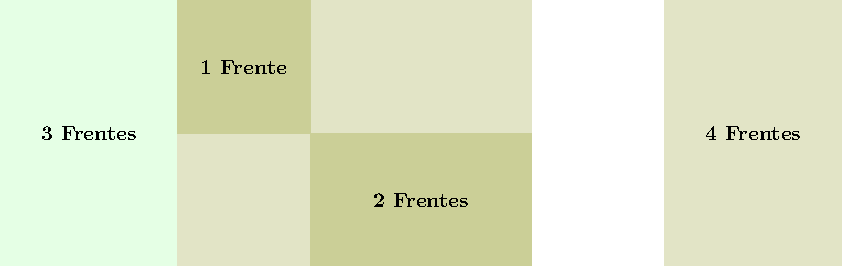
\includegraphics[width=14cm]{\rutaImagenes/frentes}
\end{figure}

\textcolor{principal}{Servicios:} es el conjunto de elementos que satisfacen las necesidades de  la vivienda  como electricidad, drenaje, telefon\'ia, agua, internet, gas entre los m\'as importantes.\\

\textcolor{principal}{Equipamiento}: Construcciones o espacios en los que se realizan actividades complementarias a las habituales como educaci\'on, cultura, salud, comercio, recreaci\'on, deporte, administraci\'on entre otros.\\

\textcolor{principal}{Infraestructura:} instalaciones necesarios para el desarrollo y funcionamiento de los municipios como transporte, vialidades, nomenclatura en  vialidades, alumbrado p\'ublico, vigilancia, etc.\\

\textcolor{principal}{Forma:}  se determina el dem\´erito con base a las caracter\'isticas del terreno como irregularidad, tama\~no del  frente o fondo ya que esto produce cierta obsolescencia funcional para la elaboraci\'on de un proyecto.\\

\textcolor{principal}{Distancia:} es la relaci\'on entre la zona centro y la ubicaci\'on de los comparables.\\

\textcolor{principal}{Tabla de ajustes}

\begin{figure}[H]
	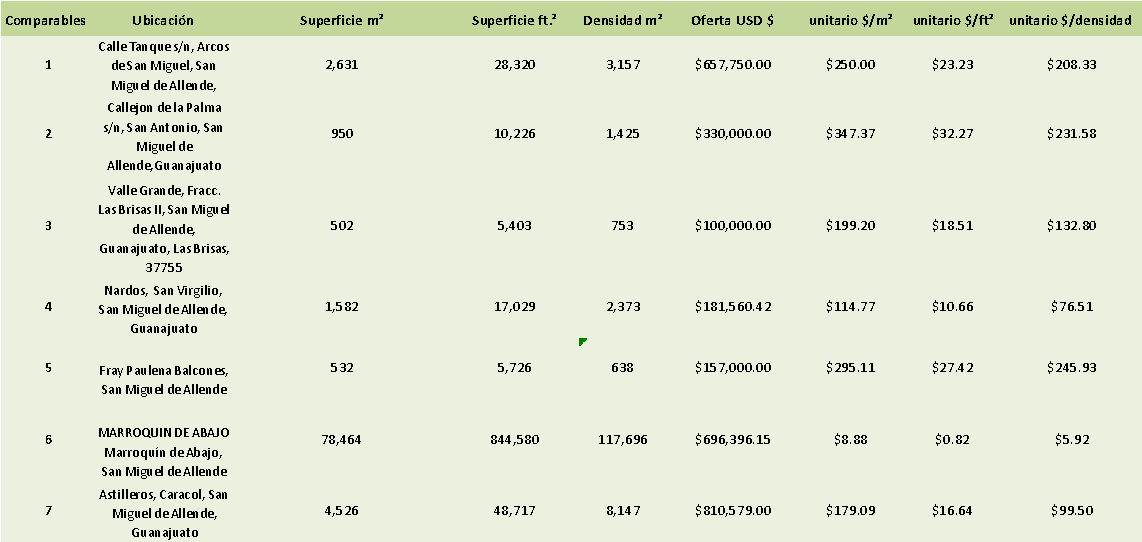
\includegraphics[width=14cm]{../0.imagenes/tabla_ajustes_1}
\end{figure}

\begin{figure}[H]
	\includegraphics[width=14cm]{../0.imagenes/tabla_ajustes_2}
\end{figure}

\begin{figure}[H]
	\includegraphics[width=7cm]{../0.imagenes/tabla_ajustes_2}
\end{figure}


Despu\'es de homologar los comparables respecto al sujeto se aplica la curva de valor para determinar el unitario por $m^2$ del valor de la tierra.\\

El factor de superficie se considera con respecto al lote tipo dentro de la zona con respecto al sujeto por lo que se concluye el valor por $m^2$ en USD \$343.05.\\

\textcolor{principal}{Metodolog\'ia 2. An\'alisis de n\'umeros enteros.}\\

Esta metodolog\'ia se aplic\'o con base a la ponderaci\'on de los comparables y la  distribuci\'on de valores a pericia del valuador y lo observado en la zona, considerando las medidas centrales para as\'i obtener el unitario por $m^2$ de tierra.\\
 
En la que se considera el valor por $m^2$ USD \$215.55.\\

\begin{figure}[H]
	\includegraphics[width=textwidth}{../0.imagenes/analisis_numeros_enteros}
\end{figure}





